\documentclass{article}
\usepackage[utf8]{inputenc}
\usepackage{graphicx}
\title{Relazione differenziale}
\author{Francesco Pio Merafina, Onofrio Davide Caputo, Alessandro Lamesta}


\begin{document}

\maketitle

\section{Abstract:}
L'esperienza della relazione consiste nell'analisi di un amplificatore differenziale, mediante la confiurazione singled ended.
~
\section{Cenni teorici:}
L'amplificatore differenziale è un amplificatore il cui scopo è quello di amplificare la differenza di due segnali in alternata. Per fare ciò si utilizza uno schema di due amplificatori BJT messi in maniera speculare in emitter comune. Una problematica di questo amplificatore è nella tensione di modo comune, cioè il segnale corrispondente al valor medio tra i due segnali, il quale è fonte di rumore. Per poter ridurre fortemente questa fonte di rumore si usa un terzo transistor in modo ad emitter comune, il quale fornirà una grande resistenza al segnale di modo comune, ma non altererà in maniera significativa l'analisi DC.
~
\begin{figure}[h!]
    \centering
    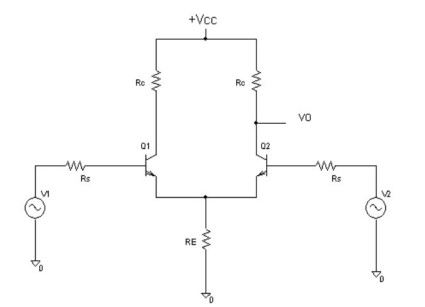
\includegraphics[width=\linewidth]{amplificatore differenziale.jpg} 
    \caption{Schema di riferimento per l'amplificatore differenziale}
    \label{figura1}
\end{figure}
~
\section{Strumentazione:}
La strumentazione utilizata per poter eseguire l'esperimento è la seguente:
\begin{itemize}
    \item generatore di tensione continua
    \item generatore di tensione alternata
    \item le seguenti resistenze con tolleranza del 5$\%$: 2 da 1.2K$\Omega$, 3 da 68K$\Omega$, 2 da 47K$\Omega$, 1 da 1K$\Omega$, 1 da 27K$\Omega$ 
    \item 5 condensatori da 47$\mu$F
    \item 1 potenziometro da 100 $\Omega$
    \item oscilloscopio
    \item 3 BJT 2N2222A
\end{itemize}
Il tutto è stato saldato su una basetta millefori, usando stagno e saldatore.
~
\section{Metodologia sperimentale e risultati:}
Come già fatto per l'amplificatore BJT, misureremo le tensioni dei  trransistor per confrontare con i valori teorici dei punti del lavoro:
\begin{table}[]
    \begin{center}
        \begin{tabular}{c|c|c|c}
        Tensione[V]&1&2&3\\
      V$_{C}$&8.90$\pm$0.50&8.89$\pm$0.46&3.30$\pm$0.02\\
      V$_{B}$&4.00$\pm$0.30&3.90$\pm$0.04&-7.40$\pm$0.06\\
      V$_{E}$&3.35$\pm$0.05&3.25$\pm$0.03&-8.00$\pm$0.04\\
      \end{tabular}
   \end{center}
\end{table} 
Successivamente si è proceduto ad effettuare le misure, prima per verificare la media banda dell'amplificatore, e poi a freqeunza fissata il guadagno.
~
\begin{table}[]
    \begin{center}
        \begin{tabular}{c|c|c|c}
        Frequenza[Hz]&V$_{i}$[mV]&V$_{o}$[mV]&Guadagno\\
        10&85$\pm$2.0&690$\pm$20&8.11$\pm$0.15\\
        30&100.0$\pm$2.0&910$\pm$20&9.10$\pm$0.21\\
        100&100$\pm$2.0&1230$\pm$20&12.30$\pm$0.23\\
        300&104$\pm$2.0&1580$\pm$20&15.19$\pm$0.19\\
        1000&106$\pm$2.0&1740$\pm$20&16.42$\pm$0.30\\
        3000&98$\pm$2.0&1800$\pm$20&18.37$\pm$0.25\\
        10000&96$\pm$2.0&1760$\pm$20&18.33$\pm$0.27\\
        30000&100$\pm$2.0&1770$\pm$20&17.70$\pm$0.30\\
        100000&102$\pm$2.0&1720$\pm$20&16.86$\pm$0.16\\
        300000&100$\pm$2.0&1740$\pm$20&17.40$\pm$0.25\\
        1000000&88$\pm$2.0&1720$\pm$20&19.55$\pm$0.17\\
        3000000&90$\pm$2.0&1450$\pm$20&16.11$\pm$0.18\\
        10000000&100$\pm$2.0&750$\pm$20&7.50$\pm$0.20\\
        \end{tabular}
   \end{center}
\end{table} 
~
\begin{table}[]
    \begin{center}
        \begin{tabular}{c|c}
        V$_{i}$[mV]&V$_{o}$[mV]\\
        24.90$\pm$2&540$\pm$10\\
        50.1$\pm$2&1015$\pm$20\\
        74.5$\pm$2&1400$\pm$20\\
        100$\pm$5&1735$\pm$20\\
        130$\pm$2&1995$\pm$20\\
        155$\pm$2&2130$\pm$20\\
        178$\pm$2&2195$\pm$20\\
        203$\pm$5&2280$\pm$20\\
        248$\pm$5&2365$\pm$20\\
        312$\pm$5&2380$\pm$20\\
        360$\pm$5&2380$\pm$20\\
        400$\pm$5&2380$\pm$20\\
        \end{tabular}
   \end{center}
\end{table} 
~
\begin{figure}[h!]
    \centering
    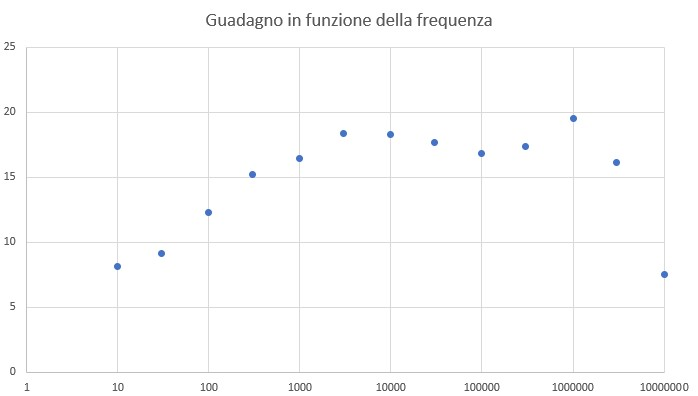
\includegraphics[width=\linewidth]{diff1.jpg} 
    \caption{Grafico del guadagno in funzione della frequenza ad ampiezza fissata}
    \label{figura1}
\end{figure}
~
\begin{figure}[h!]
    \centering
    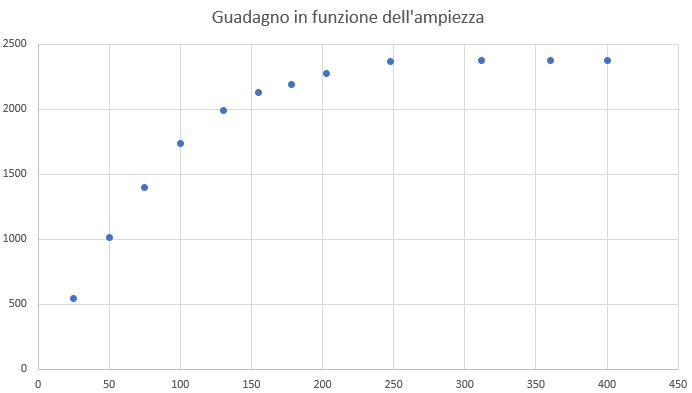
\includegraphics[width=\linewidth]{diff2.jpg} 
    \caption{Grafico del guadagno in funzione dell'ampiezza a frequenza fissata}
    \label{figura1}
\end{figure}
Per quanto riguarda il guadagno di modo comune, esso è stato attenutato fino a renderlo trascurabile, usando il poteniometro per rendere il circuito il più simmetrico possibile. 


~
\section{Conclusioni:}
In conclusione possiamo affermare che effettivamente la configurazione così montata ha un comportamento amplificante.
~
\section{Appendice:}
Testi di riferimento:
\begin{itemize}
    \item T. Floyd, Electronic devices, 9th ed. Prentice Hall
    \item Dell’Orso, Falchini, Flaminio et al. Introduzione all’elettronica digitale,
parte 2, Edizioni ETS, 2005
\end{itemize}

\end{document}